\documentclass[12pt]{article}

\usepackage{fontawesome}
\usepackage{hyperref}
\usepackage{xurl}
\usepackage{graphicx}
\usepackage{float}
\usepackage[tagged, highstructure]{accessibility}
\usepackage{bookmark}
\usepackage{enumitem}

\hypersetup{
    colorlinks=false,
    pdfborder={0 0 0},
    pdftitle={Ethics Paper},
    pdfauthor={Adrianna Holden-Gouveia},
    pdfsubject={Information Security - Lab Assignment},
    pdflang={en-US},
    pdfkeywords={computer ethics, security ethics, hacktivism, encryption, privacy}
}

% Configure PDF bookmarks for navigation
\bookmarksetup{
    numbered,
    open,
}

% Configure list spacing for better accessibility
\setlist{nosep}



\title{Ethics Paper}
\author{
        Adrianna Holden-Gouveia \\
        Website: \href{https://aholdengouveia.name}{aholdengouveia.name}\\ 
        \date{\vspace{-5ex}}
        %Email: \href{mailto:admin@aholdengouveia.name}{admin@aholdengouveia.name} \\
%        \faLinkedin{: aholdengouveia} \\
        \faGithub {: aholdengouveia} \\
        \faTwitter {: aholdengouveia} \\
        }

%S\date{\today}


\begin{document}    

\maketitle

\section*{Accessibility Notice}
This document is also available in HTML format at:

Link: \href{https://aholdengouveia.name/InfoSec/labs/ethicspaper.html}{\textbf{\nolinkurl{https://aholdengouveia.name/InfoSec/labs/ethicspaper.html}}}

The HTML version provides enhanced accessibility features including keyboard navigation, screen reader support, responsive design, dark mode support, and high contrast options.




\section*{Learning Outcomes}
By the end of this lab, you will be able to:
\begin{itemize}
    \item Research an ethical issue in computer security using reliable sources
    \item Evaluate sources with the CRAAP test, and show that each one is real
    \item Explain both sides of an ethical issue fairly, and defend your own position
    \item Connect an ethical issue to your own life and to changes in technology
\end{itemize}

\section*{Lab Instructions}
You'll write a paper of at least 2 pages about an ethical issue in computer security.

\textbf{AI rule:} AI may not be used to find sources or to write any part of this paper. Spelling and grammar checkers are fine. Submitting work that has been generated by a third party, including artificial intelligence, is strictly prohibited, and gets no credit.

\subsection*{Pick a topic}
Choose one of these topics, or something else you're interested in. If you choose your own topic, check with me first. If you've done this assignment before, you must pick a new topic. Don't turn in a paper you've already written.

Each topic is an ethical question: there's no single right answer, and reasonable people disagree. Your paper should explain the sides, and argue for your own answer.
\begin{itemize}
    \item \textbf{Hacktivism:} is it ever ethical to break into systems or leak data for a social or political cause?
    \item \textbf{Hacking back:} should companies or governments be allowed to attack the hackers who attacked them?
    \item \textbf{Encryption backdoors:} should governments be able to read encrypted messages, if it makes everyone's messages less secure?
    \item \textbf{Government tracking:} how much should governments be allowed to track people, and share that information between agencies?
    \item \textbf{Algorithms:} is it fair to let algorithms decide who gets a job, a loan, or a good social credit score?
    \item \textbf{Tracking shoppers:} is it ethical for companies to track what you buy and do online, to sell ads?
    \item \textbf{Privacy against security:} how much personal privacy should people give up to be safer?
    \item \textbf{Cyber warfare:} what are the ethical limits of cyber warfare, such as attacks that harm hospitals or other civilians?
    \item \textbf{Corporate responsibility:} how responsible should a company be when customer data is stolen?
    \item \textbf{AI in cybersecurity:} is it ethical to let AI make security decisions, such as blocking users or flagging people as threats, without a person checking?
    \item \textbf{Deepfakes:} is it ever ethical to make a deepfake of a real person without their consent?
    \item \textbf{AI training data:} is it ethical for AI companies to train their models on people's posts and personal data without asking?
    \item \textbf{AI agents:} who's responsible when an AI agent that acts on its own, without a person approving each step, causes harm?
    \item \textbf{Bug disclosure:} when someone finds a security bug, is it more ethical to tell only the company, so they can fix it first, or to tell the public?
    \item \textbf{Breach disclosure:} how quickly, and how much, should a company have to tell people after a data breach?
    \item \textbf{Schools monitoring students:} is it ethical for schools to monitor students through school-issued laptops, including at home?
    \item \textbf{Employers monitoring employees:} is it ethical for employers to read employees' email, and monitor their devices and accounts?
    \item \textbf{Health apps:} health and period-tracking apps aren't covered by HIPAA, the law that protects your medical records. Is it ethical for these companies to share or sell your health data?
    \item \textbf{Whistleblowers:} is it ethical to leak secret information to the public, as Edward Snowden did?
\end{itemize}

\subsection*{What your paper must include}
Your paper must be at least 2 pages, not counting citations, checklists, or screenshots. Include these sections, clearly labelled:
\begin{enumerate}
    \item \textbf{Statement of the problem:} the issue, in a couple of sentences.
    \item \textbf{Both sides:} explain each side of the issue. Be fair to both positions.
    \item \textbf{Your position:} give your own opinion on the ethical issue, and defend it.
    \item \textbf{A recent news article:} find a news article about your topic published in the last 3 months. Summarize it briefly, and explain why it's relevant.
    \item \textbf{Personal connection:} explain how this issue affects you, your community, a job you have or want, or something we've covered in this class. Be specific.
    \item \textbf{Looking ahead:} describe how changes in technology will affect the issue.
\end{enumerate}

\subsection*{Sources}
You need at least 5 sources, including your news article. For \textbf{each} source, include:
\begin{enumerate}
    \item A citation, in APA or MLA style. If you want to use another style, check with me first.
    \item A CRAAP test checklist or paragraph: Currency, Relevance, Authority, Accuracy, and Purpose.
    \item A screenshot of the source, showing its title and date.
    \item One direct quote from the source, and where it appears, such as the paragraph, section, or page.
\end{enumerate}
Citing in your paper:
\begin{itemize}
    \item Anything you copy word for word is a quote. Put it in quotation marks and cite it.
    \item Anything you reword, or take the ideas from, still needs a citation.
    \item Ideas you've put together from several sources in your own words don't need a citation in the sentence, but the sources must be in your source list.
\end{itemize}

\subsection*{Screenshots}
Each screenshot should have your name, term, and year.  One of the easiest ways to do that is make a text document with your name and term/year on your computer and save it to use all term. Any screenshots that don't include this information won't be counted.

\begin{figure}[H]
    \centerline{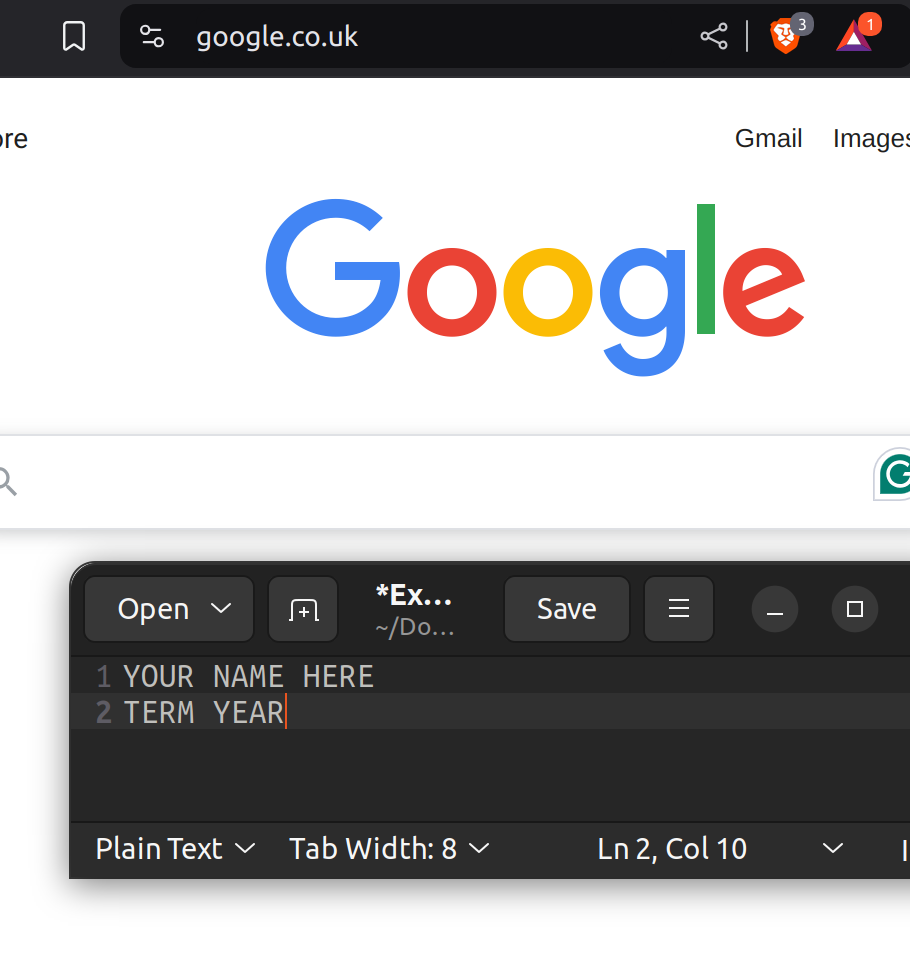
\includegraphics[scale=.2]{ExampleScreenshot.png}}
    \caption{This is an image of what each of your screenshots should look like}
    \alt{Example screenshot: a web browser showing the Google home page, with a small text editor window in front of it that says YOUR NAME HERE and TERM YEAR}
\end{figure}

\section*{Deliverables}
One file that includes:
\begin{itemize}
    \item Your paper, with all 6 sections clearly labelled
    \item Your source list, with a CRAAP check, a screenshot, and a direct quote for each source
\end{itemize}
The CRAAP checks, screenshots, and quotes can go at the end of your paper.

\section*{Resources}
References, a video, a PowerPoint and some notes are available at my website
Link: \href{https://www.aholdengouveia.name/InfoSec/Ethics.html}{\textbf{\nolinkurl{https://www.aholdengouveia.name/InfoSec/Ethics.html}}}

My guide to evaluating sources
Link: \href{https://www.aholdengouveia.name/Howtos/Sourceeval/sourceEvaluation.html}{\textbf{\nolinkurl{https://www.aholdengouveia.name/Howtos/Sourceeval/sourceEvaluation.html}}}

The CRAAP test, with questions to ask about each source
Link: \href{https://web.archive.org/web/20250814000638/https://guides.lib.uchicago.edu/c.php?g=1241077&p=9082343}{\textbf{\nolinkurl{https://web.archive.org/web/20250814000638/https://guides.lib.uchicago.edu/c.php?g=1241077&p=9082343}}}

Another explanation of the CRAAP test
Link: \href{https://libguides.butler.edu/c.php?g=117303&p=1940068}{\textbf{\nolinkurl{https://libguides.butler.edu/c.php?g=117303&p=1940068}}}

\end{document}